\documentclass[full-course-notes.tex]{subfiles}

\begin{document}
\lecturemeta{8}
  {The Landscape of Parsing; Context-Free Grammars and Derivations; Grammar Engineering:
   Left Factoring and Left Recursion}
  {CLO 1, CLO 2}
  {\S4.1 (Introduction to Syntax Analysis: top-down vs.\ bottom-up), \S4.2 (Context-Free
   Grammars: derivations, parse trees), \S4.3.3 (Elimination of Left Recursion), \S4.3.4
   (Left Factoring)}
  {[ET] Engineering a Compiler, \S3.1--3.2; [AP] Modern Compiler Implementation, Ch.\,3}
\lecshort{Parsing Overview; CFGs; Left Recursion \& Left Factoring}
\setcounter{section}{0}
\makelecturetitle

\begin{coreidea}[Lecture Roadmap]
\begin{enumerate}
  \item A \textbf{bird's-eye map of parsing}: every parsing algorithm this course will ever
  name falls under either \textbf{top-down} or \textbf{bottom-up} construction of a parse
  tree, and every algorithm's one-line ``key feature'' is worth knowing before we build any of
  them in depth.
  \item \textbf{Context-free grammars (CFGs)}: the formalism parsing needs, precisely because
  Lecture~\ref{lec:4} already showed regular expressions cannot express nested structure.
  \item \textbf{Derivations and parse trees}: what it formally means to ``generate'' a string
  from a grammar, worked through on one running example.
  \item \textbf{Grammar engineering, part 1 -- Left Factoring}: why sharing a common prefix
  between productions is a real problem for a predictive parser, and how to remove it.
  \item \textbf{Grammar engineering, part 2 -- Left Recursion}: a \emph{different}, more severe
  problem specifically for top-down parsers, and how to remove it -- both the simple (direct)
  and general (indirect) cases.
\end{enumerate}
This is deliberately a \emph{first} lecture on parsing: a map of the territory and the grammar
hygiene every later algorithm assumes has already been done, not yet any actual parsing
algorithm. The lectures ahead build the leaves of today's tree one at a time, in depth.
\end{coreidea}

\section{The Landscape of Parsing}
\label{sec:l8-landscape}

\dbtag Lecture~\ref{lec:2}'s phase pipeline (\Sref{sec:l2-phase-pipeline}) named
\textbf{syntax analysis} as the phase right after lexical analysis: it takes the token stream
and organizes it into a \textbf{parse tree} (or \textbf{syntax tree}) reflecting the program's
grammatical structure. Every algorithm that does this job falls into exactly one of two
families, distinguished by \emph{which end of the parse tree it builds first}.

\begin{defbox}{Top-Down vs.\ Bottom-Up Parsing}
\begin{itemize}
  \item A \textbf{top-down} parser builds the parse tree starting at the \textbf{root} (the
  grammar's start symbol) and works \emph{downward} toward the leaves (the actual input
  tokens), at every point guessing/deriving which production to expand next so that the
  eventual leaves match the input.
  \item A \textbf{bottom-up} parser builds the parse tree starting at the \textbf{leaves} (the
  input tokens themselves) and works \emph{upward}, repeatedly recognizing a piece of the input
  that matches the right-hand side of some production and collapsing it into that production's
  left-hand side, until only the start symbol remains.
\end{itemize}
Both families are guaranteed to produce the \emph{same} parse tree for an unambiguous grammar
on a given input -- they differ only in the \emph{order} in which that one tree gets
constructed, which turns out to have major consequences for which grammars each family can
handle and how each is implemented.
\end{defbox}

\begin{center}
\resizebox{\textwidth}{!}{%
\begin{tikzpicture}[
  level distance=2.0cm,
  every node/.style={draw, thick, rounded corners, minimum width=2.6cm, minimum height=0.9cm,
                      align=center, font=\small},
  level 1/.style={sibling distance=19cm},
  level 2/.style={sibling distance=4.4cm},
  level 3/.style={sibling distance=2.8cm},
  edge from parent/.style={draw, thick, -{Latex}}
]
\node[fill=nuLight, draw=nuNavy] {Parsing\\(build the parse tree)}
  child { node[fill=dbGreenBg, draw=dbGreen] {Top-Down\\root $\to$ leaves}
    child { node[fill=dbGreenBg!60, draw=dbGreen] {Backtracking\\(try, undo, retry)} }
    child { node[fill=dbGreenBg, draw=dbGreen] {Predictive\\(no backtracking)}
      child { node[fill=dbGreenBg!60, draw=dbGreen] {Recursive-\\Descent} }
      child { node[fill=dbGreenBg!60, draw=dbGreen] {LL(1)\\(table-driven)} }
      child { node[fill=dbGreenBg!60, draw=dbGreen] {LL($*$)\\(ANTLR, adaptive)} }
    }
  }
  child { node[fill=examRedBg, draw=examRed] {Bottom-Up\\leaves $\to$ root}
    child { node[fill=examRedBg, draw=examRed] {Shift-Reduce:\\the LR Family}
      child { node[fill=examRedBg!60, draw=examRed] {LR(0)} }
      child { node[fill=examRedBg!60, draw=examRed] {SLR(1)} }
      child { node[fill=examRedBg!60, draw=examRed] {LALR(1)} }
      child { node[fill=examRedBg!60, draw=examRed] {CLR(1)\\(canonical LR)} }
    }
    child { node[fill=examRedBg!60, draw=examRed] {Operator-\\Precedence} }
    child { node[fill=examRedBg!60, draw=examRed] {Universal\\(CYK, Earley)} }
  }
;
\end{tikzpicture}}
\end{center}

\begin{center}
\renewcommand{\arraystretch}{1.35}
\small
\begin{tabularx}{\textwidth}{@{}l l X@{}}
\toprule
\textbf{Family} & \textbf{Algorithm} & \textbf{One-Line Key Feature} \\
\midrule
Top-down & Backtracking & Tries a production, and if it leads to a dead end, undoes the choice
and tries the next one -- simple to describe, but can cost exponential time in the worst case;
essentially never used in production compilers. \\
Top-down & Recursive-Descent & One hand-written function per nonterminal, calling other such
functions to match the right-hand side -- simple, flexible, easy to add custom error messages
to, but \emph{requires} a grammar with no left recursion and no unresolved left factors
(\Sref{sec:l8-left-factoring}--\Sref{sec:l8-left-recursion}). \\
Top-down & LL(1) & A \emph{mechanically constructed} parsing table, built from FIRST/FOLLOW
sets, driven by a generic stack-based simulation loop -- ``LL'' = read input Left-to-right,
produce a Leftmost derivation, using 1 token of lookahead. \\
Top-down & LL($*$) & A modern relative of LL(1) that adaptively looks ahead as many tokens as
needed (not just one) to decide between productions -- what ANTLR4 actually builds; more
grammars accepted than plain LL(1), at the cost of a more complex parser generator. \\
Bottom-up & LR(0) & The base LR automaton, built from ``items'' with \emph{no} lookahead at all
-- rarely used directly (it accepts very few grammars), but it is the foundation SLR(1),
LALR(1), and CLR(1) all extend with progressively richer lookahead. \\
Bottom-up & SLR(1) & ``Simple LR'': the smallest, easiest-to-build LR table, using the LR(0)
automaton plus FOLLOW sets to decide when to reduce -- but the weakest lookahead-equipped
member of the LR family, rejecting some genuinely unambiguous grammars. \\
Bottom-up & LALR(1) & Merges canonical LR(1) states that share the same core -- same (small)
table size as SLR(1), but strictly more grammars accepted; the industry-standard algorithm
(what Yacc/Bison actually build). \\
Bottom-up & CLR(1) & ``Canonical LR(1)'': keeps every LR(1) state distinct, with full
per-state lookahead -- the most powerful of the three, accepting the largest class of grammars,
but with tables that can be dramatically larger, which is exactly why LALR(1) is preferred in
practice. \\
Bottom-up & Operator-Precedence & An older, simpler technique that only ranks operators against
each other (no full grammar automaton needed) -- easy to hand-build for expression grammars,
but far less general than the LR family; largely superseded by LR parsing today. \\
Bottom-up & Universal (CYK, Earley) & General-purpose algorithms that can parse \emph{any}
context-free grammar (even ambiguous ones), using dynamic programming -- CYK needs the grammar
in a normal form and runs in $O(n^3)$; Earley handles arbitrary CFGs directly. Too slow for
everyday compiler use, but standard in NLP parsing and grammar-tooling contexts where
generality matters more than raw speed. \\
\bottomrule
\end{tabularx}
\end{center}

\begin{examfocus}
Memorize the shape of this tree, not just the list of names: \textbf{every} bottom-up algorithm
in this course is a member of the \textbf{shift-reduce} family (they all maintain a stack and
decide, at each step, whether to \emph{shift} the next input symbol onto the stack or
\emph{reduce} the stack's top symbols using a production) -- SLR(1), LALR(1), and CLR(1) differ
\emph{only} in how much lookahead information their tables encode, not in the shift-reduce
mechanism itself. This is exactly the kind of ``classify this algorithm'' question that shows
up on exams: given an algorithm's name, you should be able to place it correctly on this tree
without hesitation.
\end{examfocus}

\begin{coreidea}[What's a Preview, and What's a Full Build]
Today you are seeing every leaf of this tree \emph{by name only} -- a bird's-eye key feature,
nothing more. The lectures ahead build several of these leaves in full mechanical detail (how
to construct a FIRST/FOLLOW-based LL(1) table; how to build an LR(0) automaton and extend it to
SLR(1), then LALR(1), with a brief look at canonical LR(1)) -- but before any of that
construction can begin, every grammar first needs two specific problems fixed. That is the
second half of today's lecture.
\end{coreidea}

\section{Context-Free Grammars}
\label{sec:l8-cfg}

\dbtag Lecture~\ref{lec:4}'s \Sref{sec:l4-regular-vs-nonregular} already proved the gap this
section fills: regular expressions have no way to \emph{count} an unbounded quantity, which is
exactly why balanced parentheses -- and, by the same argument, the nested structure of every
real programming language's expressions, blocks, and function calls -- cannot be expressed with
a regular expression. A \textbf{context-free grammar (CFG)} is the more powerful formalism that
\emph{can} express this nesting, and it is the formalism every parser in
\Sref{sec:l8-landscape}'s tree is built to process.

\begin{defbox}{Context-Free Grammar}
A context-free grammar is a 4-tuple $(N, T, P, S)$ where:
\begin{itemize}
  \item $N$ is a finite set of \textbf{nonterminals} -- syntactic categories like
  \texttt{expr} or \texttt{stmt} that stand for a set of strings, not any one fixed string;
  \item $T$ is a finite set of \textbf{terminals} -- the actual tokens coming out of the lexer
  (\Sref{sec:l3-tokens-patterns-lexemes}), disjoint from $N$;
  \item $P$ is a finite set of \textbf{productions}, each of the form $A \to \alpha$ where
  $A \in N$ and $\alpha \in (N \cup T)^{*}$ -- ``nonterminal $A$ can be replaced by the string
  $\alpha$''; several productions for the same $A$ are usually written together as
  $A \to \alpha_1 \mid \alpha_2 \mid \dots$;
  \item $S \in N$ is the \textbf{start symbol}, the one nonterminal every derivation begins
  from.
\end{itemize}
\end{defbox}

\begin{examplebox}{A Running Example: Simple Arithmetic Expressions}
This grammar for \texttt{+}, \texttt{*}, parentheses, and \texttt{id} will be reused for every
worked example in the rest of this lecture:
\begin{center}
\ttfamily
\begin{tabular}{@{}l@{}}
$E \to E + T \mid T$ \\
$T \to T * F \mid F$ \\
$F \to ( E ) \mid \texttt{id}$
\end{tabular}
\end{center}
Here $N = \{E, T, F\}$, $T_{\text{terminals}} = \{\texttt{+}, \texttt{*}, (, ), \texttt{id}\}$,
and the start symbol is $E$. Notice the grammar already encodes operator precedence
structurally: $T$ (a ``term'') can only ever appear as a \texttt{+}-separated piece of $E$, and
$F$ (a ``factor'') can only appear as a \texttt{*}-separated piece of $T$ -- multiplication is
forced to bind tighter than addition purely by \emph{which nonterminal contains which}, with no
explicit precedence numbers anywhere.
\end{examplebox}

\section{Derivations and Parse Trees}
\label{sec:l8-derivations}

\begin{defbox}{Derivation}
A \textbf{derivation} is a sequence of production applications, starting from the start symbol
$S$, that rewrites one nonterminal at a time until only terminals remain. Each intermediate
string (a mix of terminals and nonterminals) is a \textbf{sentential form}. A
\textbf{leftmost derivation} always rewrites the \emph{leftmost} remaining nonterminal at every
step; a \textbf{rightmost derivation} always rewrites the \emph{rightmost} one. (Both are valid,
equally correct ways to generate the \emph{same} string -- they simply commit to a fixed order
so the derivation is unambiguous to describe, and different parser families naturally correspond
to one or the other, as \Sref{sec:l8-landscape}'s LL/LR naming already hinted.)
\end{defbox}

\begin{examplebox}{Worked Example: Leftmost Derivation of \texttt{id + id * id}}
Using \Sref{sec:l8-cfg}'s expression grammar:
\begin{center}
\renewcommand{\arraystretch}{1.25}
\small
\begin{tabular}{@{}lll@{}}
$E$ & $\Rightarrow E + T$ & ($E \to E + T$) \\
& $\Rightarrow T + T$ & ($E \to T$) \\
& $\Rightarrow F + T$ & ($T \to F$) \\
& $\Rightarrow \texttt{id} + T$ & ($F \to \texttt{id}$) \\
& $\Rightarrow \texttt{id} + T * F$ & ($T \to T * F$) \\
& $\Rightarrow \texttt{id} + F * F$ & ($T \to F$) \\
& $\Rightarrow \texttt{id} + \texttt{id} * F$ & ($F \to \texttt{id}$) \\
& $\Rightarrow \texttt{id} + \texttt{id} * \texttt{id}$ & ($F \to \texttt{id}$) \\
\end{tabular}
\end{center}
At every step, the \emph{leftmost} nonterminal in the current sentential form is the one
rewritten -- notice how the parenthesization implied by precedence (multiplication grouped
under one $T$) falls straight out of \emph{which} nonterminal gets expanded, never out of any
explicit precedence rule.
\end{examplebox}

\begin{center}
\resizebox{!}{4.3cm}{%
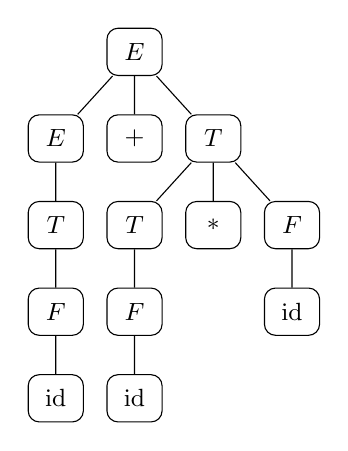
\begin{tikzpicture}[
  level distance=11mm,
  sibling distance=10mm,
  every node/.style={draw, rounded corners, minimum width=7mm, minimum height=6mm, align=center, font=\small}
]
\node {$E$}
  child { node {$E$}
    child { node {$T$}
      child { node {$F$}
        child { node {id} }
      }
    }
  }
  child { node {$+$} }
  child { node {$T$}
    child { node {$T$}
      child { node {$F$}
        child { node {id} }
      }
    }
    child { node {$*$} }
    child { node {$F$}
      child { node {id} }
    }
  }
;
\end{tikzpicture}}
\end{center}
\begin{center}
\small\textit{The parse tree for \texttt{id + id * id}: exactly the tree the leftmost
derivation above builds, one production per internal node. Reading the leaves left to right
reproduces the original input string -- this ``yield'' property holds for \emph{any} valid
parse tree, top-down or bottom-up.}
\end{center}

\begin{examfocus}
A single parse tree corresponds to \emph{many} different derivation orders (leftmost,
rightmost, or anything in between) -- the tree is the ground truth; a derivation is just one
particular order of announcing it. Do not confuse ``two different derivations'' with ``two
different parse trees'': the former can happen for a perfectly ordinary, unambiguous grammar
(swap which nonterminal you expand first); the latter -- genuinely different \emph{trees} for
the \emph{same} string -- is what \textbf{ambiguity} means, and is the subject of the next
lecture, not this one.
\end{examfocus}

\section{Grammar Engineering, Part 1: Left Factoring}
\label{sec:l8-left-factoring}

\dbtag A top-down parser -- whether hand-written recursive descent or a generated LL(1) table
-- has to decide \emph{which production to use} for the current nonterminal by looking at only
a small, fixed amount of upcoming input (for LL(1), exactly \emph{one} token). That decision
becomes impossible whenever two productions for the same nonterminal start the same way.

\begin{defbox}{Left Factoring}
A grammar has a \textbf{left factor} (a common prefix) when some nonterminal $A$ has two or
more productions $A \to \alpha\beta_1 \mid \alpha\beta_2 \mid \dots$ that begin with the same
nonempty string $\alpha$. \textbf{Left factoring} is the grammar transformation that rewrites
these into $A \to \alpha A' $ and $A' \to \beta_1 \mid \beta_2 \mid \dots$ -- deferring the
decision of \emph{which} $\beta_i$ until after $\alpha$ has already been matched and a new
nonterminal $A'$ is reached, at which point enough input has been consumed to decide correctly.
\end{defbox}

\begin{coreidea}[Why Common Prefixes Arise, and Why They're a Real Problem]
Shared prefixes are not a rare, contrived situation -- they show up naturally wherever a
language offers an \emph{optional trailing clause} on top of a shorter, complete construct.
DB's classic example: an \texttt{if} statement with an \emph{optional} \texttt{else} --
\texttt{if expr then stmt} is already a complete statement on its own, but
\texttt{if expr then stmt else stmt} is also legal, and the two productions share the entire
prefix \texttt{if expr then stmt}. A predictive parser reading left to right cannot know, right
after matching \texttt{then stmt}, whether it should be using the first production or the
second -- both are still equally plausible until the \emph{next} token (\texttt{else}, or
something else) actually arrives. Left uncorrected, the parser is left with exactly two bad
options, and both cost real time on \emph{every single} parse, not just pathological ones:
\begin{enumerate}
  \item \textbf{Backtracking} -- guess a production, and if a later mismatch reveals the guess
  was wrong, undo everything done so far and try the next production. This can require
  re-scanning already-processed input, repeatedly, and in the worst case costs exponential
  time (\Sref{sec:l8-landscape}'s ``Backtracking'' row).
  \item \textbf{Extra lookahead} -- peek further ahead than one token to decide, which not only
  slows down \emph{every} parsing step (not just the ambiguous ones) but can require
  arbitrarily much lookahead for some grammars, defeating the whole point of a simple,
  fixed-lookahead table-driven parser.
\end{enumerate}
Left factoring sidesteps both costs entirely: after the transformation, one token of lookahead
is always enough, because the parser is never asked to choose between competing productions
until they have actually diverged.
\end{coreidea}

\begin{examplebox}{Worked Example 1: The Classic \texttt{if}/\texttt{else}}
\begin{center}
\ttfamily
\begin{tabular}{@{}l@{}}
Before: \\
$\text{stmt} \to \texttt{if } expr \texttt{ then } stmt$ \\
$\phantom{\text{stmt} \to} \mid \texttt{if } expr \texttt{ then } stmt \texttt{ else } stmt$ \\
$\phantom{\text{stmt} \to} \mid \text{other}$ \\[4pt]
After (common prefix $\texttt{if } expr \texttt{ then } stmt$ factored out): \\
$\text{stmt} \to \texttt{if } expr \texttt{ then } stmt\ stmt' \mid \text{other}$ \\
$stmt' \to \texttt{else } stmt \mid \varepsilon$
\end{tabular}
\end{center}
Every string the original grammar could generate, the new grammar still generates -- left
factoring changes \emph{how} a string is derived, never \emph{which} strings are in the
language. A predictive parser can now decide correctly: after matching
\texttt{if expr then stmt}, it peeks at the next token; if it's \texttt{else}, use
$stmt' \to \texttt{else } stmt$; otherwise, use $stmt' \to \varepsilon$ and move on. (This is
also exactly the classic ``dangling else'' ambiguity in disguise -- the next lecture returns to
it from the ambiguity angle specifically.)
\end{examplebox}

\begin{examplebox}{Worked Example 2: A Smaller, Purely Mechanical Case}
\begin{center}
\ttfamily
\begin{tabular}{@{}ll@{}}
Before: & $A \to \texttt{a}A_1 \mid \texttt{a}A_2 \mid \texttt{a}A_3$ \\
After: & $A \to \texttt{a}A' \qquad A' \to A_1 \mid A_2 \mid A_3$
\end{tabular}
\end{center}
The common prefix here is the single terminal \texttt{a}; factoring it out leaves the new
nonterminal $A'$ to decide among $A_1$, $A_2$, $A_3$ using whatever token comes \emph{after}
the \texttt{a} -- exactly one token further than the original grammar could safely commit to.
\end{examplebox}

\begin{examfocus}
Left factoring sometimes has to be applied \textbf{more than once}: factoring out one common
prefix can expose a \emph{new} common prefix one level deeper (e.g.\ if $A_1$ and $A_2$ above
themselves both started with the same symbol). DB's algorithm is understood to repeat until no
nonterminal has any left-factorable productions left -- checking once and stopping is a common
exam and implementation mistake.
\end{examfocus}

\section{Grammar Engineering, Part 2: Left Recursion}
\label{sec:l8-left-recursion}

\dbtag A second, unrelated grammar property is just as disqualifying for top-down parsing --
but for a completely different, more severe reason than left factoring's slowdown.

\begin{defbox}{Left Recursion}
A grammar is \textbf{immediately left-recursive} if some nonterminal $A$ has a production of
the form $A \to A\alpha$ -- $A$'s own right-hand side begins with $A$ itself. More generally, a
grammar is (\textbf{indirectly}) left-recursive if $A \Rightarrow^{+} A\alpha$ for \emph{some}
sequence of production applications, for some string $\alpha$ -- $A$ eventually derives
something beginning with $A$ again, possibly by passing through several \emph{other}
nonterminals first, not just directly.
\end{defbox}

\begin{coreidea}[Why Left Recursion Is Worse Than a Slowdown: Infinite Loops]
Recall \Sref{sec:l8-landscape}'s recursive-descent row: a top-down parser calls one function
per nonterminal, and to parse $A$ it calls \texttt{parseA()}. If $A \to A\alpha$ is one of
$A$'s productions, then \texttt{parseA()}'s very first action -- \emph{before consuming a
single input token} -- is to call \texttt{parseA()} again, to match that leading $A$. That
inner call does exactly the same thing, calling \texttt{parseA()} once more, and so on
forever: the recursion never bottoms out, because no input is ever consumed to make progress
toward a base case. The concrete result is unbounded recursion and a stack overflow, not merely
a slow parse. This is the precise, mechanical reason left recursion and left factoring are
\emph{both} grammar-engineering steps every top-down technique requires, yet are fundamentally
different kinds of problems:
\end{coreidea}

\begin{center}
\renewcommand{\arraystretch}{1.4}
\begin{tabularx}{\textwidth}{@{}l X X@{}}
\toprule
 & \textbf{Left Factoring
 (\Sref{sec:l8-left-factoring})} & \textbf{Left Recursion (here)} \\
\midrule
\textbf{Symptom} & Two or more productions for the same nonterminal share a common prefix &
Some nonterminal, directly or indirectly, has a production whose right-hand side starts with
itself \\
\textbf{What goes wrong for a top-down parser} & Cannot choose which production to use with
only one token of lookahead & Cannot make \emph{any} progress at all before recursing again \\
\textbf{Consequence if left unfixed} & Forced into backtracking or extra lookahead -- a real,
but bounded, performance cost & Unbounded recursion -- the parser \textbf{never terminates}
(stack overflow), regardless of the input \\
\textbf{Severity} & A performance / parser-design problem & A \textbf{correctness} problem --
the parser is simply broken for this grammar \\
\bottomrule
\end{tabularx}
\end{center}

\begin{examfocus}
A very common exam confusion: describing left recursion as ``making the parser slow,'' the same
language used for left factoring. Be precise -- left recursion does not slow a top-down parser
down, it makes it \textbf{not terminate at all} for a naive implementation. Bottom-up (LR-family)
parsers, by contrast, have \emph{no} problem with left recursion at all -- in fact left-recursive
grammars are often \emph{preferred} for LR parsing, since they keep the parser's stack bounded
where an equivalent right-recursive grammar would not. Left recursion is specifically a
\textbf{top-down} problem, not a universal one.
\end{examfocus}

\subsection{Eliminating Immediate Left Recursion}
\label{sec:l8-left-recursion-immediate}

\begin{coreidea}[The Standard Transformation]
Given $A \to A\alpha_1 \mid A\alpha_2 \mid \dots \mid A\alpha_m \mid \beta_1 \mid \beta_2 \mid
\dots \mid \beta_n$, where none of the $\beta_i$ themselves start with $A$, rewrite as:
\[
A \to \beta_1 A' \mid \beta_2 A' \mid \dots \mid \beta_n A' \qquad\qquad
A' \to \alpha_1 A' \mid \alpha_2 A' \mid \dots \mid \alpha_m A' \mid \varepsilon
\]
In words: every alternative that \emph{doesn't} start with $A$ (a $\beta_i$) becomes a starting
point, immediately followed by a new nonterminal $A'$; every alternative that \emph{did} start
with $A$ (an $\alpha_i$) becomes a \emph{tail}, hung off $A'$ instead, with $A'$ itself allowed
to be empty. The recursion has not disappeared -- it has simply been converted from
\emph{left}-recursion into \emph{right}-recursion (every recursive call to $A'$ now comes
\emph{after} consuming some real input), which top-down parsing has no trouble with at all.
\end{coreidea}

\begin{examplebox}{Worked Example: Removing Left Recursion From the Expression Grammar}
Applying the transformation to \Sref{sec:l8-cfg}'s running example, nonterminal by nonterminal:
\begin{center}
\ttfamily
\begin{tabular}{@{}ll@{}}
Before: & $E \to E + T \mid T$ \qquad\qquad ($\alpha_1 = {}+T$, $\beta_1 = T$) \\
After: & $E \to T E' \qquad E' \to {+} T E' \mid \varepsilon$ \\[6pt]
Before: & $T \to T * F \mid F$ \qquad\qquad ($\alpha_1 = {}*F$, $\beta_1 = F$) \\
After: & $T \to F T' \qquad T' \to {*} F T' \mid \varepsilon$ \\[6pt]
Unchanged: & $F \to ( E ) \mid \texttt{id}$ \qquad ($F$ was never left-recursive)
\end{tabular}
\end{center}
The resulting grammar generates \emph{exactly} the same language as before, but a
\texttt{parseE()} function built from it now consumes at least one token (via
\texttt{parseT()}) before ever calling \texttt{parseE'()} -- the infinite-regress problem from
the coreidea box above is gone by construction.
\end{examplebox}

\subsection{Eliminating Indirect (General) Left Recursion}
\label{sec:l8-left-recursion-indirect}

\dbtag Left recursion can hide across \emph{several} nonterminals, with no single production
obviously guilty on its own -- $A$ may not start with $A$ anywhere in the grammar as written,
yet still derive something starting with $A$ once other nonterminals are expanded. The general
algorithm handles this in exactly the two steps the immediate case already gave us, just with
one extra step in front: \textbf{first turn the indirect recursion into direct (immediate)
recursion by substitution, then eliminate that immediate recursion exactly as in
\Sref{sec:l8-left-recursion-immediate}.}

\begin{coreidea}[DB Algorithm 4.19 -- General Left-Recursion Elimination]
\begin{enumerate}
  \item \textbf{Order the nonterminals} arbitrarily: $A_1, A_2, \dots, A_n$.
  \item \textbf{For $i = 1$ to $n$:}
  \begin{enumerate}[label=(\alph*)]
    \item \textbf{Substitute (make direct).} For each $j < i$, replace every production of the
    form $A_i \to A_j\gamma$ with one copy of $A_i \to \delta\gamma$ for \emph{every} current
    production $A_j \to \delta$ of $A_j$ -- literally pasting $A_j$'s right-hand sides in where
    $A_j$ used to sit. Because $j < i$, $A_j$ has already been fully processed by this point
    (its own left recursion, if any, is already gone), so this substitution cannot reintroduce
    a recursion through $A_j$ -- it can only ever convert a recursion \emph{through} an earlier
    nonterminal into a \emph{direct} recursion on $A_i$ itself.
    \item \textbf{Eliminate (remove it).} Apply
    \Sref{sec:l8-left-recursion-immediate}'s standard transformation to whatever $A_i$'s
    productions have become after step (a), exactly as if it had been immediately
    left-recursive from the start.
  \end{enumerate}
\end{enumerate}
The two-step shape of the inner loop is the whole idea: \textbf{(a) substitute until the
recursion is directly visible, (b) then remove it with the one formula we already have.} No new
elimination technique is needed -- indirect left recursion is only ever a substitution step
away from being the immediate case.
\end{coreidea}

\begin{examplebox}{Worked Example 1: DB's Classic Two-Nonterminal Case}
\begin{center}
\ttfamily
$S \to A\texttt{a} \mid \texttt{b} \qquad\qquad A \to A\texttt{c} \mid S\texttt{d} \mid
\varepsilon$
\end{center}
Order the nonterminals $S$ (=$A_1$), then $A$ (=$A_2$).

\textbf{$i=1$ ($S$):} no $j < 1$, so no substitution is possible yet. Checking $S$'s own
productions, $S \to A\texttt{a} \mid \texttt{b}$ does not start with $S$ -- already free of
immediate left recursion. $S$ is left unchanged.

\textbf{$i=2$ ($A$), step (a) -- substitute:} $A$'s production $A \to S\texttt{d}$ starts with
the earlier nonterminal $S$, so replace it with one copy per $S$-production: $S \to A\texttt{a}$
gives $A\texttt{a}\texttt{d}$, and $S \to \texttt{b}$ gives $\texttt{b}\texttt{d}$. Combined with
$A$'s other, unaffected productions ($A\texttt{c}$ and $\varepsilon$, neither of which started
with $S$), $A$'s production set is now:
\[
A \to A\texttt{c} \mid A\texttt{a}\texttt{d} \mid \texttt{b}\texttt{d} \mid \varepsilon
\]
This \emph{is} now immediately left-recursive -- exactly the point of step (a).

\textbf{$i=2$ ($A$), step (b) -- eliminate:} Matching \Sref{sec:l8-left-recursion-immediate}'s
template with $\alpha_1 = \texttt{c}$, $\alpha_2 = \texttt{a}\texttt{d}$ (the two
$A$-starting alternatives) and $\beta_1 = \texttt{b}\texttt{d}$, $\beta_2 = \varepsilon$ (the
two that don't start with $A$):
\[
A \to \texttt{b}\texttt{d}A' \mid A' \qquad\qquad A' \to \texttt{c}A' \mid
\texttt{a}\texttt{d}A' \mid \varepsilon
\]
\textbf{Final grammar} (left-recursion-free, same language as the original):
\[
S \to A\texttt{a} \mid \texttt{b} \qquad A \to \texttt{b}\texttt{d}A' \mid A' \qquad A' \to
\texttt{c}A' \mid \texttt{a}\texttt{d}A' \mid \varepsilon
\]
\end{examplebox}

\begin{examplebox}{Worked Example 2: Mutual Recursion With No $\varepsilon$-Production}
A second case, to see the same two steps on a grammar shaped slightly differently -- here $A$
and $B$ recurse through each other directly, with no ``escape hatch'' production like the
$\varepsilon$ above:
\begin{center}
\ttfamily
$A \to B\texttt{a} \mid \texttt{c} \qquad\qquad B \to A\texttt{b} \mid \texttt{d}$
\end{center}
Order $A$ (=$A_1$), then $B$ (=$A_2$).

\textbf{$i=1$ ($A$):} no $j<1$; $A \to B\texttt{a} \mid \texttt{c}$ does not start with $A$ --
unchanged.

\textbf{$i=2$ ($B$), step (a) -- substitute:} $B$'s production $B \to A\texttt{b}$ starts with
the earlier nonterminal $A$, so substitute $A$'s productions in: $A \to B\texttt{a}$ gives
$B\texttt{a}\texttt{b}$, and $A \to \texttt{c}$ gives $\texttt{c}\texttt{b}$. Combined with $B$'s
unaffected production ($\texttt{d}$), $B$'s production set becomes:
\[
B \to B\texttt{a}\texttt{b} \mid \texttt{c}\texttt{b} \mid \texttt{d}
\]
Immediately left-recursive, exactly as intended.

\textbf{$i=2$ ($B$), step (b) -- eliminate:} With $\alpha_1 = \texttt{a}\texttt{b}$ and
$\beta_1 = \texttt{c}\texttt{b}$, $\beta_2 = \texttt{d}$:
\[
B \to \texttt{c}\texttt{b}B' \mid \texttt{d}B' \qquad\qquad B' \to \texttt{a}\texttt{b}B' \mid
\varepsilon
\]
\textbf{Final grammar:}
\[
A \to B\texttt{a} \mid \texttt{c} \qquad B \to \texttt{c}\texttt{b}B' \mid \texttt{d}B' \qquad
B' \to \texttt{a}\texttt{b}B' \mid \varepsilon
\]
Notice the new nonterminal $B'$ appears \emph{only} because $B$ needed it -- substitution alone
never by itself requires a new nonterminal; only the elimination step (b) ever introduces one,
exactly as in the immediate case.
\end{examplebox}

\begin{examfocus}
Every instance of indirect left-recursion elimination is these same two steps, in this order,
never the other way around: \textbf{substitute first} (using only already-processed, earlier
nonterminals) \textbf{to expose direct recursion, then eliminate} it with
\Sref{sec:l8-left-recursion-immediate}'s one formula. Trying to ``eliminate'' before the
recursion is direct is not meaningful -- there is no left-recursive alternative to apply the
formula to until substitution has produced one. You are responsible for executing \emph{both}
steps correctly on a small (two- or three-nonterminal) example, the way both worked examples
above did.
\end{examfocus}

\section{Self-Check Questions}
\label{sec:l8-selfcheck}

\begin{enrichment}[Practice -- Not Graded]
\begin{enumerate}
  \item Given only the algorithm name ``CLR(1),'' place it correctly on
  \Sref{sec:l8-landscape}'s tree (top-down or bottom-up? which sub-family?) and state its
  one-line key feature from memory.
  \item Write the 4-tuple $(N, T, P, S)$ explicitly for a small grammar of your own choosing
  that generates balanced parentheses, $\{a^n b^n \mid n \ge 0\}$-style. (Lecture~\ref{lec:4}'s
  \Sref{sec:l4-regular-vs-nonregular} already showed this language is \emph{not} regular --
  confirm for yourself that a two-production CFG handles it easily.)
  \item Using \Sref{sec:l8-cfg}'s expression grammar, write out the \emph{rightmost} derivation
  of \texttt{id * id + id} (note: different string, different operator order, from the
  leftmost-derivation example in the lecture).
  \item Left-factor the grammar $A \to \texttt{c}A\texttt{d} \mid \texttt{c}B \mid B\texttt{e}$
  where the shared prefix is only between the \emph{first two} alternatives. Show your work.
  \item Explain, without using the word ``slow,'' exactly what goes wrong -- mechanically, in a
  recursive-descent function -- when a grammar is left-recursive. Contrast this precisely with
  what goes wrong when a grammar merely has unfactored common prefixes.
  \item Eliminate immediate left recursion from
  $S \to S + S \mid S * S \mid \texttt{id}$. (This grammar is also ambiguous -- you are not
  asked to fix that here, only to mechanically apply
  \Sref{sec:l8-left-recursion-immediate}'s transformation and confirm the result is no longer
  left-recursive.)
  \item Apply \Sref{sec:l8-left-recursion-indirect}'s general algorithm to
  $X \to Y\texttt{c} \mid \texttt{e}$, $Y \to X\texttt{d} \mid Y\texttt{f} \mid \texttt{g}$
  (order $X$ before $Y$). Show the substitution step (a) and the resulting
  immediate-left-recursion elimination step (b) as two clearly separate stages, the way both
  worked examples in this lecture did -- this grammar is deliberately a little richer than
  either worked example (step (a) here feeds \emph{two} $Y$-alternatives into step (b), not
  just one).
\end{enumerate}
\end{enrichment}

\begin{takeaways}
\begin{itemize}
  \item Every parsing algorithm in this course is either \textbf{top-down} (root $\to$ leaves)
  or \textbf{bottom-up} (leaves $\to$ root); every bottom-up algorithm covered here is a
  \textbf{shift-reduce}, LR-family algorithm, differing only in how much lookahead its table
  encodes (SLR(1) $\subsetneq$ LALR(1) $\subsetneq$ CLR(1) in grammars accepted).
  \item A \textbf{context-free grammar} is exactly the formalism regular expressions cannot
  provide: the ability to express unbounded, nested structure, via nonterminals and recursive
  productions.
  \item A \textbf{derivation} rewrites the start symbol one nonterminal at a time down to pure
  terminals; a \textbf{parse tree} is the resulting structure, and many different derivation
  \emph{orders} (leftmost, rightmost, \dots) can all produce the very same tree.
  \item \textbf{Left factoring} removes shared prefixes between productions so a predictive
  parser can always decide which production to use with a small, fixed amount of lookahead --
  skipping it forces either costly backtracking or ever-growing lookahead.
  \item \textbf{Left recursion} is a stricter, correctness-level problem specific to top-down
  parsing: a left-recursive nonterminal's parsing function recurses before consuming any input,
  which never terminates. The standard transformation converts left recursion into right
  recursion without changing the language generated -- first for the \textbf{immediate} case,
  then, when needed, via the general algorithm for \textbf{indirect} left recursion.
  \item Left factoring and left recursion are \textbf{independent} problems, fixed by
  \textbf{independent} transformations -- a grammar can have either, both, or neither, and both
  must be resolved before any of \Sref{sec:l8-landscape}'s top-down algorithms can be built on
  top of it.
\end{itemize}
\end{takeaways}

\section*{References for This Lecture}
\begin{thebibliography}{99}
\bibitem[DB]{db} Aho, A.~V., Lam, M.~S., Sethi, R., and Ullman, J.~D. \textit{Compilers:
Principles, Techniques, and Tools}. 2nd~ed. Pearson, 2006.
\bibitem[ET]{et} Cooper, K.~D. and Torczon, L. \textit{Engineering a Compiler}. 2nd~ed. Morgan
Kaufmann, 2011.
\bibitem[AP]{ap} Appel, A.~W. \textit{Modern Compiler Implementation in C/Java/ML}. Cambridge
University Press, 2004.
\end{thebibliography}

\end{document}
